\documentclass[aspectratio=169]{beamer}
\mode<presentation>
%\usetheme{Warsaw}
%\usetheme{Goettingen}
\usetheme{Hannover}
%\useoutertheme{default}

%\useoutertheme{infolines}
\useoutertheme{sidebar}
\usecolortheme{dolphin}


\setbeamersize{sidebar width left=0pt} % to remove the sidebar
\beamertemplatenavigationsymbolsempty % To remove the navigation symbols on the bottom right.
\setbeamersize{text margin left=10mm,text margin right=10mm} % Specify margins

\usepackage{amsmath}
\usepackage{amssymb}
\usepackage{listings}
\usepackage{enumerate}
\usepackage{hyperref}
\hypersetup{
    colorlinks=true,
    linkcolor=blue,
    filecolor=magenta,      
    urlcolor=cyan,
}
 
\urlstyle{same}

%some bold math symbosl
\newcommand{\Cov}{\mathrm{Cov}}
\newcommand{\Var}{\mathrm{Var}}
\newcommand{\brho}{\boldsymbol{\rho}}
\newcommand{\bSigma}{\boldsymbol{\Sigma}}
\newcommand{\btheta}{\boldsymbol{\theta}}
\newcommand{\bbeta}{\boldsymbol{\beta}}
\newcommand{\bmu}{\boldsymbol{\mu}}
\newcommand{\bW}{\mathbf{W}}
\newcommand{\one}{\mathbf{1}}
\newcommand{\bH}{\mathbf{H}}
\newcommand{\by}{\mathbf{y}}
\newcommand{\bolde}{\mathbf{e}}
\newcommand{\bx}{\mathbf{x}}

\newcommand{\cpp}[1]{\texttt{#1}}

%--------------------------------------------------
\providecommand{\abs}[1]{\lvert#1\rvert}
\providecommand{\norm}[1]{\lVert#1\rVert}
\providecommand{\Blue}[1]{\textcolor{blue}{#1}}
\providecommand{\Red}[1]{\textcolor{red}{#1}}
\newcommand{\celsius}{\ensuremath{^\circ}C}
\newcommand\thfore{\mathord{\therefore}\,}
%------------------------------------------------------------------

\title{Lecture 26. Basics Counting Operations in Algorithms}

%\author{\includegraphics[width=.7\textwidth,height=.7\textheight]{lecture20-fig0.png}}

\date{ }
\vspace{.5in}

%------------------------------------------------------------------


\begin{document}

\frame[plain]{\titlepage}

%%%%%%%%%%%%%%%%%%
\iffalse
\begin{frame}[plain]{Counting}

{\bf Activity 20.1}. How many bit strings of length four start with 1 or end with 00?
 %https://ggc-discrete-math.github.io/counting.html#_counting    Example 7

\vspace{2.5in}

\end{frame}

\fi
%%%%%%%%%%%%%%%%%%%%%%%%%%%%
 


\begin{frame}[plain]{Loop}

	{\bf Example 26.1.} What is the total number of additions performed by the
		code?
		  \begin{center}
		  	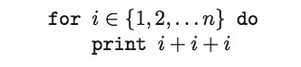
\includegraphics[height=1.3cm]{./img/lecture26-fig1.png}
		  \end{center}
   \pause
   
   	
	{\bf Multiplication Principle for Algorithms.} If {\bf STATEMENT} 
		 requires \Blue{$m$} of a certain type 
		of operation, then a \Blue{loop} that repeats {\bf STATEMENT} \Blue{$n$}
		times requires \Blue{$mn$} operations.

	
	\vspace{.5in}
	
\end{frame}

%\begin{frame}[plain]{}

% {\bf Activity 20.2}. What will be the value '\texttt{\Blue{counter}(10, 9,  7, 10, 5)}' 
% when the following code is run?
    
%    \begin{center}
%			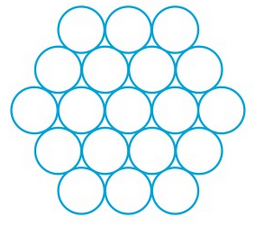
\includegraphics[height=4cm]{lecture20-fig3.png} 
%	\end{center}
	
	
%	\vspace{.5in}
	
%\end{frame}

\begin{frame}[plain]{}


 {\bf Example 26.2}. Let $A$ be the set of 26 letters of alphabet. 
		  Interpret the following algorithm and count 
		  how many strings does it print?
		  
	\begin{center}
			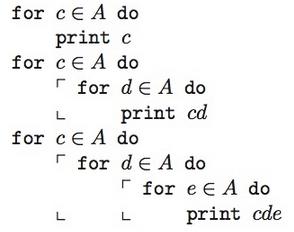
\includegraphics[height=4cm]{./img/lecture26-fig2.png} 
	\end{center}
 \medskip

%Answer: $26+26^2+26^3$
\vspace{.5in}

 		
 
 % {\bf Example 19.2.} Assume $A$ has $m$ elements and $B$ has $n$ elements.
 %		How many comparisons does this code perform? 		   
 %		\begin{center}
 %			\includegraphics[height=1.5cm]{lecture20-fig6.png}
 %		\end{center}


\end{frame}



\begin{frame}[plain]{Array}
	
{\small 
		An \Blue{array} is a sequence of variables $x_1, x_2, x_3, ..., x_n$; e.g., 
		 \begin{center}
		 	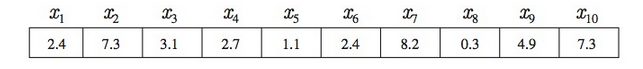
\includegraphics[height=1cm]{./img/lecture26-fig3.png}
		 \end{center}
	Notice that the order of the elements in an array matters.%, and an array can have duplicate entries.
	\pause
		 \medskip
		 
		{\bf Example 26.3.} The following algorithm counts the number of duplicates
		  in the array $x_1, x_2, ..., x_n$, where $n>1$. How many "=" comparisons does the algorithm perform? For example, 
		when $x_1=20, x_2=50, x_3=50, x_4=18$.  (Use the trace table of the algorithm.)
		  \begin{columns}
		  \begin{column}{0.5\textwidth}
		\begin{center}
			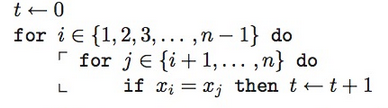
\includegraphics[height=1.7cm]{./img/lecture26-fig4.png} 
		\end{center}		
		 \end{column}
		 \begin{column}{0.5\textwidth}
		   \centering
		   
		   \vspace{0.7in}
		 \end{column}
		 \end{columns}
	}
	\vspace{.5in}
	
	
\end{frame}

\begin{frame}[plain]{}
 
 \begin{center}
   {\bf \Blue{Trace} of the algorithm in Example 26.3}\\ 
    \smallskip 
    
   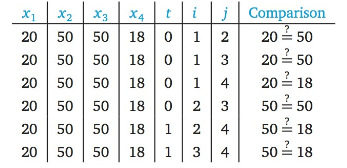
\includegraphics[height=3cm]{./img/lecture26-fig5.png}
 \end{center}
 
 The number of comparisons is evidently  3+2+1=6 in this case. In general, this algorithm will make
 \[ \Blue{ S_n = (n-1)+(n-2)+\cdots +2+1 = \pause  \frac{n(n-1)}{2} \in \ 
     \mbox{Big-}\Theta(n^2) } \]
     
  {\bf Remark}. If $S_n \leq \frac{n(n-1)}{2}$ , then we say \Blue{$S_n\in \mathcal{O}(n^2)$}.
  If $S_n \geq \frac{n(n-1)}{2}$ , then we say \Blue{$S_n\in \Omega(n^2)$}.
 
 \end{frame}
 
 \begin{frame}[plain]{}
 
 {\bf Practice 26.4.}  Consider the same algorithm in Example 25.3.
 \begin{center}
			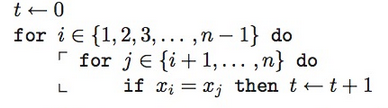
\includegraphics[height=1.7cm]{./img/lecture26-fig4.png} 
		\end{center}
 
  Let $x_1=10, x_2=20, x_3=30, x_4=20, x_5=10$. When tracing the algorithm, 
  choose the right sequence of $t$ in order. 
 
 %[PollEv.com/bongsikkim470]
 \vspace{1in}
 %Answer for  19.5-2: $t = 0, 0, 0, 1, 1, 2, 2, 2, 2, 2$
  
\end{frame}


\begin{frame}[plain]{Sorting}
 A \Blue{sort} is an algorithm that guarantees that
	       \[ x_1\leq  x_2\leq  x_3\leq \cdots \leq x_n \]
	       after the algorithm finishes.\pause 
	       \smallskip
	       
 {\bf Example 26.5.} Let $x_1, x_2, ..., x_n$ be an array whose elements can be compared
		    by $\leq $. The following algorithm is called a \Blue{bubble sort}.
		    Step through this algorithm for the list $x_1=9, x_2=4, x_3=7$, and $x_4=1$.
		How many times does it make the ``$>$'' comparison when sorting a list of $n$ 
		elements?
		\begin{columns}
		\begin{column}{0.5\textwidth}
		\begin{center}
			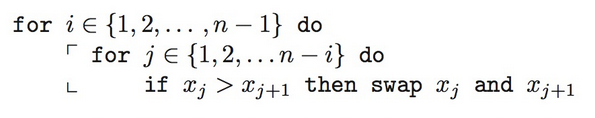
\includegraphics[height=1.3cm]{./img/lecture26-fig6.png}
			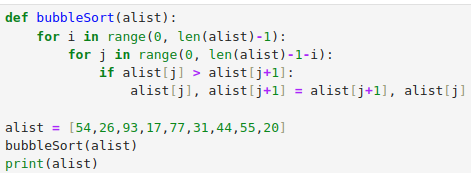
\includegraphics[height=2.2cm]{./img/lecture26-fig6b.png}
		\end{center}
		\vspace{1.5in}
		
		\end{column}
		\begin{column}{0.5\textwidth}		   
		   
		 \end{column}
		 \end{columns}

\end{frame}

\begin{frame}[plain]{}
 
  \begin{center}
   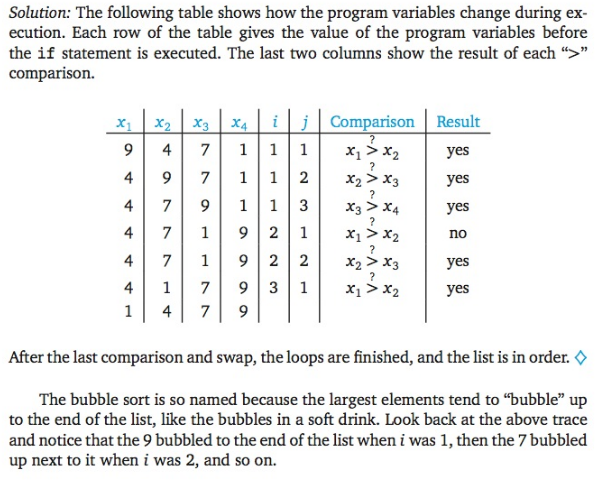
\includegraphics[height=7cm]{lecture26-fig7.png}
  \end{center}
  The `if' statement requires one comparison. The outside loop makes the inside loop execute $n-1$ times,
  but each time the size of the index set for $j$ gets smaller. Thus, the total number of comparisons is
  \Blue{$(n-1)+(n-2)+\cdots +2+1 = \frac{n(n-1)}{2} \in \ \mbox{Big-}\Theta(n^2)$}.
 
\end{frame}

\begin{frame}[plain]{}

  {\bf Practice 26.6.}   Trace through the bubble sort algorithm for the following data set.
     \[ x_1 = 5, x_2=4, x_3=2, x_4=1, x_5=3. \]
     %Essentials (3rd), Exercises 4.5 #21 on p282
     
     \begin{center}
			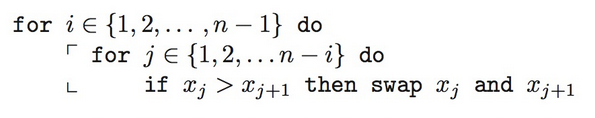
\includegraphics[height=1.7cm]{./img/lecture26-fig6.png}
		\end{center}
  \vspace{1in}
  
\end{frame}

\end{document}

%%%%%%%%%%%%%%%%%%%%%%%%%%%%%%%%%%%%%%%%%%%%%%%%%%%

\begin{frame}[plain]{Exercises}

  \begin{enumerate}
   \item A startup with four employee rents an office suite with seven offices. 
    How many ways are there to assign the employees?
   \item Let $n>3$. Consider the following pseudocode segment.
   
       \begin{center}
			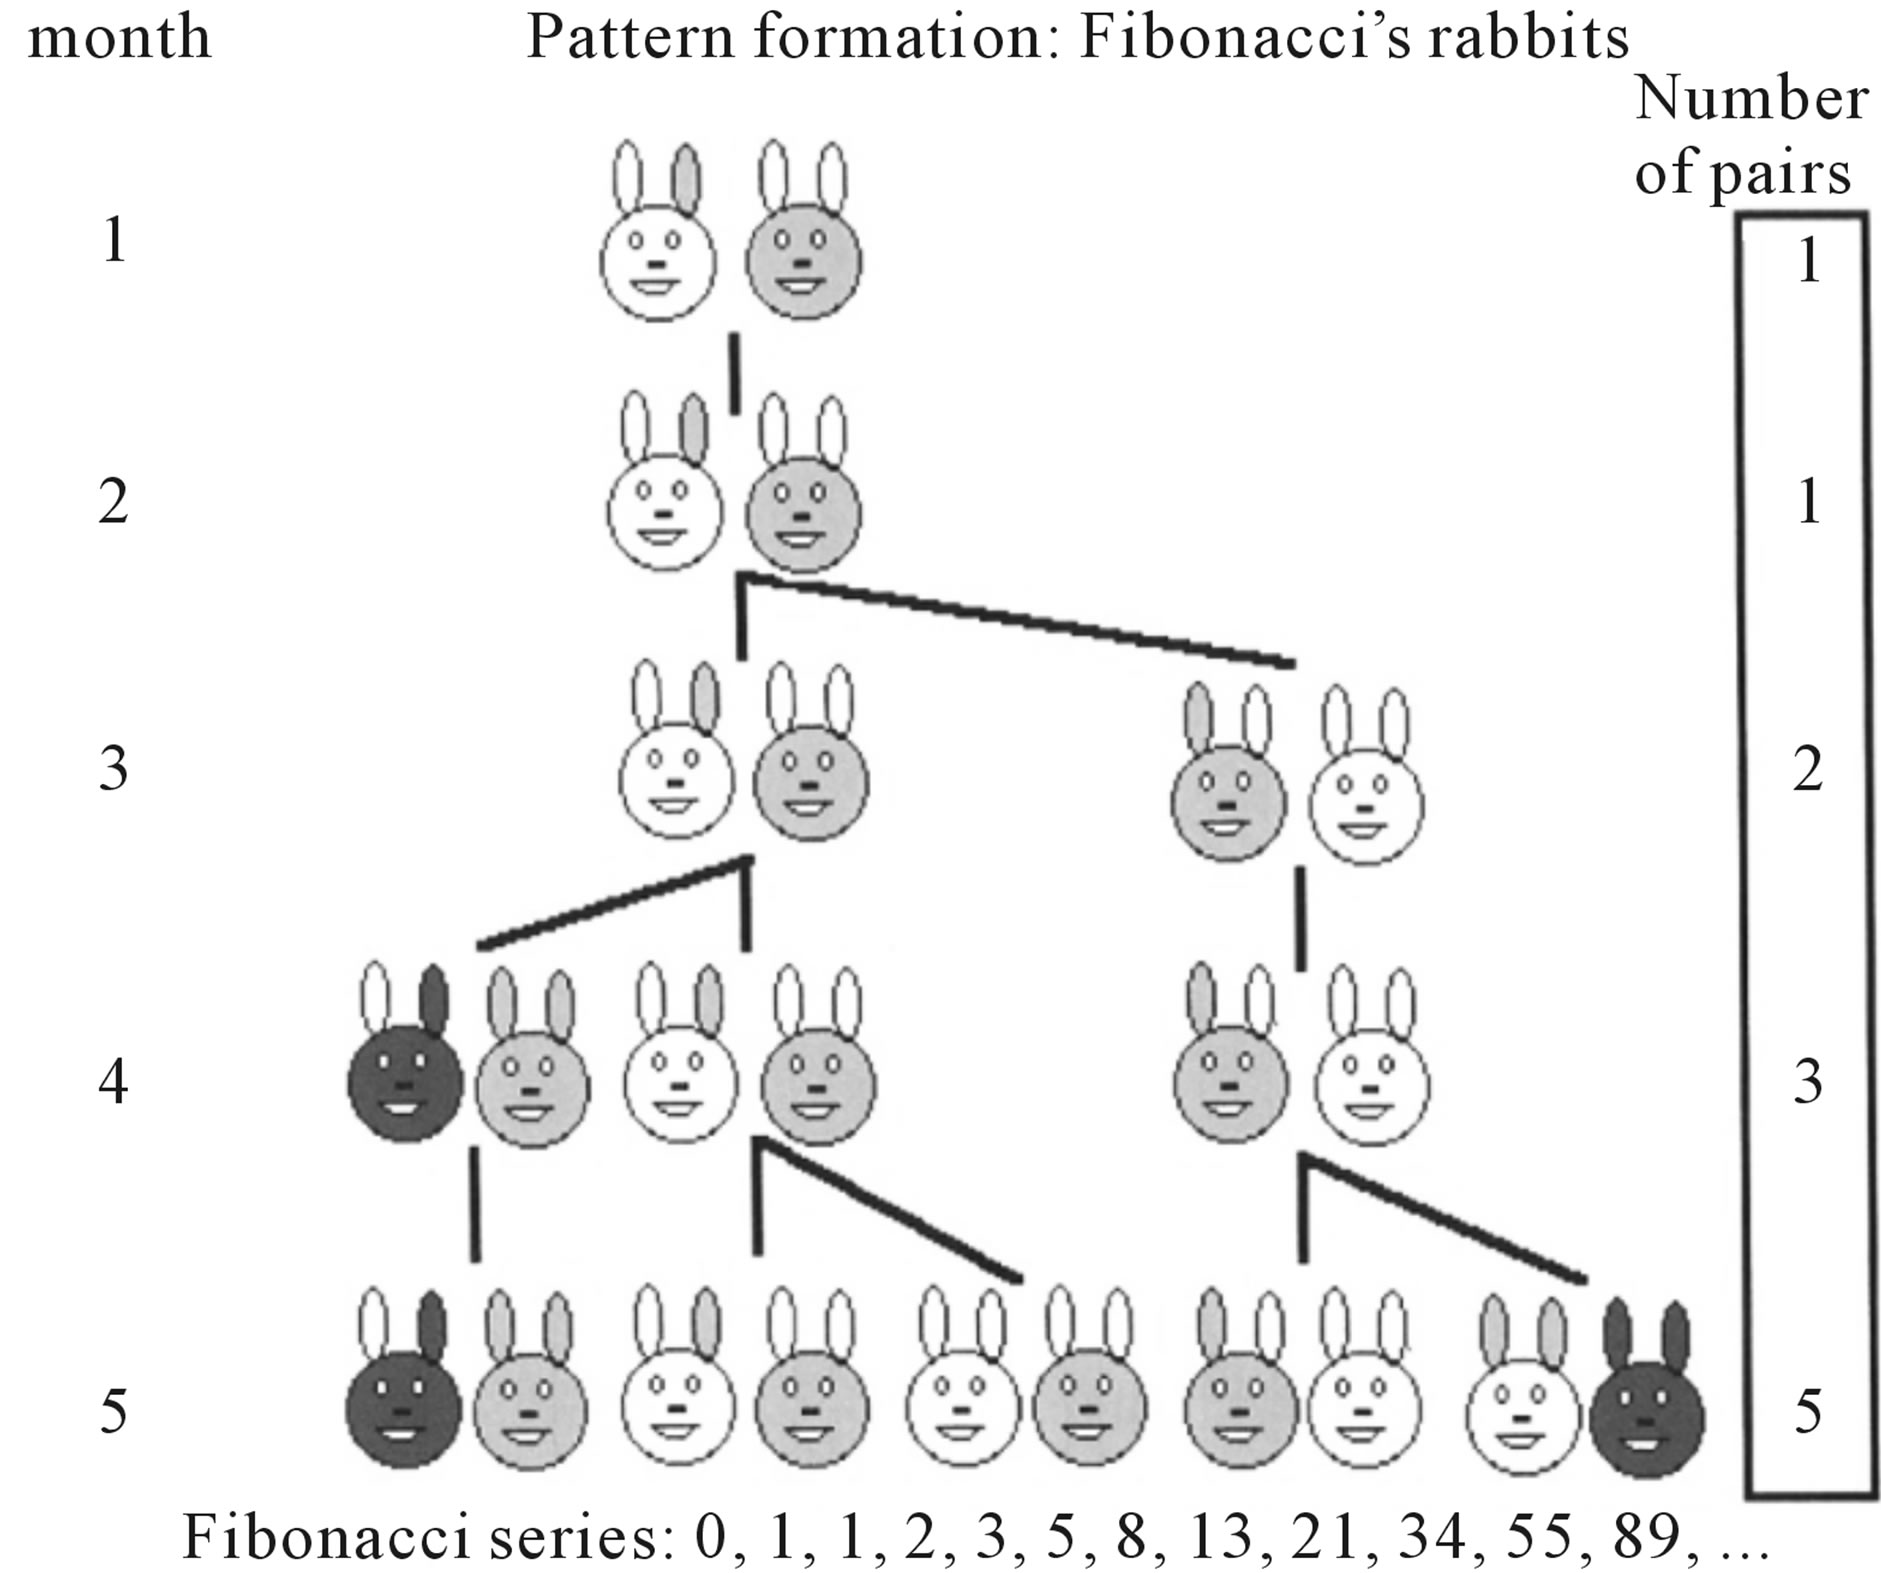
\includegraphics[height=3.3cm]{lecture20-fig1.png}
		\end{center}
		How many "+" operations does this algorithm perform?
		%Essentials (3rd), Exercises 4.5 #11 on p280
   \item If a card is drawn from a standard 52-card deck,
    how many ways can the card be black or a face card?

  \end{enumerate}

\end{frame}

\begin{frame}[plain]{}

  \begin{enumerate}
   \setcounter{enumi}{3}

  \item Let $x_1, x_2, ..., x_n$ be an array whose elements can be compared 
    by the total ordering $\leq$. 
    \begin{itemize}
      \item[(a)] Write an algorithm for computing the maximum element in the array. 
      \item[(b)] How many ``$<$" comparisons does your algorithm require?
      \item[(c)] Write a python code based on your algorithm and test your assertion in (b) with   
    examples of several arrays.
   \end{itemize}
    %https://github.com/bkimo/discrete-math-with-python/blob/master/lab2-bubble-sort.ipynb
  \end{enumerate}

\end{frame}








\end{document}

